\documentclass[11pt]{article}

    \usepackage[breakable]{tcolorbox}
    \usepackage{parskip} % Stop auto-indenting (to mimic markdown behaviour)

    \usepackage{iftex}
    \ifPDFTeX
    	\usepackage[T1]{fontenc}
    	\usepackage{mathpazo}
    \else
    	\usepackage{fontspec}
    \fi

    % Basic figure setup, for now with no caption control since it's done
    % automatically by Pandoc (which extracts ![](path) syntax from Markdown).
    \usepackage{graphicx}
    % Maintain compatibility with old templates. Remove in nbconvert 6.0
    \let\Oldincludegraphics\includegraphics
    % Ensure that by default, figures have no caption (until we provide a
    % proper Figure object with a Caption API and a way to capture that
    % in the conversion process - todo).
    \usepackage{caption}
    \DeclareCaptionFormat{nocaption}{}
    \captionsetup{format=nocaption,aboveskip=0pt,belowskip=0pt}

    \usepackage{float}
    \floatplacement{figure}{H} % forces figures to be placed at the correct location
    \usepackage{xcolor} % Allow colors to be defined
    \usepackage{enumerate} % Needed for markdown enumerations to work
    \usepackage{geometry} % Used to adjust the document margins
    \usepackage{amsmath} % Equations
    \usepackage{amssymb} % Equations
    \usepackage{textcomp} % defines textquotesingle
    % Hack from http://tex.stackexchange.com/a/47451/13684:
    \AtBeginDocument{%
        \def\PYZsq{\textquotesingle}% Upright quotes in Pygmentized code
    }
    \usepackage{upquote} % Upright quotes for verbatim code
    \usepackage{eurosym} % defines \euro
    \usepackage[mathletters]{ucs} % Extended unicode (utf-8) support
    \usepackage{fancyvrb} % verbatim replacement that allows latex
    \usepackage{grffile} % extends the file name processing of package graphics
                         % to support a larger range
    \makeatletter % fix for old versions of grffile with XeLaTeX
    \@ifpackagelater{grffile}{2019/11/01}
    {
      % Do nothing on new versions
    }
    {
      \def\Gread@@xetex#1{%
        \IfFileExists{"\Gin@base".bb}%
        {\Gread@eps{\Gin@base.bb}}%
        {\Gread@@xetex@aux#1}%
      }
    }
    \makeatother
    \usepackage[Export]{adjustbox} % Used to constrain images to a maximum size
    \adjustboxset{max size={0.9\linewidth}{0.9\paperheight}}

    % The hyperref package gives us a pdf with properly built
    % internal navigation ('pdf bookmarks' for the table of contents,
    % internal cross-reference links, web links for URLs, etc.)
    \usepackage{hyperref}
    % The default LaTeX title has an obnoxious amount of whitespace. By default,
    % titling removes some of it. It also provides customization options.
    \usepackage{titling}
    \usepackage{longtable} % longtable support required by pandoc >1.10
    \usepackage{booktabs}  % table support for pandoc > 1.12.2
    \usepackage[inline]{enumitem} % IRkernel/repr support (it uses the enumerate* environment)
    \usepackage[normalem]{ulem} % ulem is needed to support strikethroughs (\sout)
                                % normalem makes italics be italics, not underlines
    \usepackage{mathrsfs}



    % Colors for the hyperref package
    \definecolor{urlcolor}{rgb}{0,.145,.698}
    \definecolor{linkcolor}{rgb}{.71,0.21,0.01}
    \definecolor{citecolor}{rgb}{.12,.54,.11}

    % ANSI colors
    \definecolor{ansi-black}{HTML}{3E424D}
    \definecolor{ansi-black-intense}{HTML}{282C36}
    \definecolor{ansi-red}{HTML}{E75C58}
    \definecolor{ansi-red-intense}{HTML}{B22B31}
    \definecolor{ansi-green}{HTML}{00A250}
    \definecolor{ansi-green-intense}{HTML}{007427}
    \definecolor{ansi-yellow}{HTML}{DDB62B}
    \definecolor{ansi-yellow-intense}{HTML}{B27D12}
    \definecolor{ansi-blue}{HTML}{208FFB}
    \definecolor{ansi-blue-intense}{HTML}{0065CA}
    \definecolor{ansi-magenta}{HTML}{D160C4}
    \definecolor{ansi-magenta-intense}{HTML}{A03196}
    \definecolor{ansi-cyan}{HTML}{60C6C8}
    \definecolor{ansi-cyan-intense}{HTML}{258F8F}
    \definecolor{ansi-white}{HTML}{C5C1B4}
    \definecolor{ansi-white-intense}{HTML}{A1A6B2}
    \definecolor{ansi-default-inverse-fg}{HTML}{FFFFFF}
    \definecolor{ansi-default-inverse-bg}{HTML}{000000}

    % common color for the border for error outputs.
    \definecolor{outerrorbackground}{HTML}{FFDFDF}

    % commands and environments needed by pandoc snippets
    % extracted from the output of `pandoc -s`
    \providecommand{\tightlist}{%
      \setlength{\itemsep}{0pt}\setlength{\parskip}{0pt}}
    \DefineVerbatimEnvironment{Highlighting}{Verbatim}{commandchars=\\\{\}}
    % Add ',fontsize=\small' for more characters per line
    \newenvironment{Shaded}{}{}
    \newcommand{\KeywordTok}[1]{\textcolor[rgb]{0.00,0.44,0.13}{\textbf{{#1}}}}
    \newcommand{\DataTypeTok}[1]{\textcolor[rgb]{0.56,0.13,0.00}{{#1}}}
    \newcommand{\DecValTok}[1]{\textcolor[rgb]{0.25,0.63,0.44}{{#1}}}
    \newcommand{\BaseNTok}[1]{\textcolor[rgb]{0.25,0.63,0.44}{{#1}}}
    \newcommand{\FloatTok}[1]{\textcolor[rgb]{0.25,0.63,0.44}{{#1}}}
    \newcommand{\CharTok}[1]{\textcolor[rgb]{0.25,0.44,0.63}{{#1}}}
    \newcommand{\StringTok}[1]{\textcolor[rgb]{0.25,0.44,0.63}{{#1}}}
    \newcommand{\CommentTok}[1]{\textcolor[rgb]{0.38,0.63,0.69}{\textit{{#1}}}}
    \newcommand{\OtherTok}[1]{\textcolor[rgb]{0.00,0.44,0.13}{{#1}}}
    \newcommand{\AlertTok}[1]{\textcolor[rgb]{1.00,0.00,0.00}{\textbf{{#1}}}}
    \newcommand{\FunctionTok}[1]{\textcolor[rgb]{0.02,0.16,0.49}{{#1}}}
    \newcommand{\RegionMarkerTok}[1]{{#1}}
    \newcommand{\ErrorTok}[1]{\textcolor[rgb]{1.00,0.00,0.00}{\textbf{{#1}}}}
    \newcommand{\NormalTok}[1]{{#1}}

    % Additional commands for more recent versions of Pandoc
    \newcommand{\ConstantTok}[1]{\textcolor[rgb]{0.53,0.00,0.00}{{#1}}}
    \newcommand{\SpecialCharTok}[1]{\textcolor[rgb]{0.25,0.44,0.63}{{#1}}}
    \newcommand{\VerbatimStringTok}[1]{\textcolor[rgb]{0.25,0.44,0.63}{{#1}}}
    \newcommand{\SpecialStringTok}[1]{\textcolor[rgb]{0.73,0.40,0.53}{{#1}}}
    \newcommand{\ImportTok}[1]{{#1}}
    \newcommand{\DocumentationTok}[1]{\textcolor[rgb]{0.73,0.13,0.13}{\textit{{#1}}}}
    \newcommand{\AnnotationTok}[1]{\textcolor[rgb]{0.38,0.63,0.69}{\textbf{\textit{{#1}}}}}
    \newcommand{\CommentVarTok}[1]{\textcolor[rgb]{0.38,0.63,0.69}{\textbf{\textit{{#1}}}}}
    \newcommand{\VariableTok}[1]{\textcolor[rgb]{0.10,0.09,0.49}{{#1}}}
    \newcommand{\ControlFlowTok}[1]{\textcolor[rgb]{0.00,0.44,0.13}{\textbf{{#1}}}}
    \newcommand{\OperatorTok}[1]{\textcolor[rgb]{0.40,0.40,0.40}{{#1}}}
    \newcommand{\BuiltInTok}[1]{{#1}}
    \newcommand{\ExtensionTok}[1]{{#1}}
    \newcommand{\PreprocessorTok}[1]{\textcolor[rgb]{0.74,0.48,0.00}{{#1}}}
    \newcommand{\AttributeTok}[1]{\textcolor[rgb]{0.49,0.56,0.16}{{#1}}}
    \newcommand{\InformationTok}[1]{\textcolor[rgb]{0.38,0.63,0.69}{\textbf{\textit{{#1}}}}}
    \newcommand{\WarningTok}[1]{\textcolor[rgb]{0.38,0.63,0.69}{\textbf{\textit{{#1}}}}}


    % Define a nice break command that doesn't care if a line doesn't already
    % exist.
    \def\br{\hspace*{\fill} \\* }
    % Math Jax compatibility definitions
    \def\gt{>}
    \def\lt{<}
    \let\Oldtex\TeX
    \let\Oldlatex\LaTeX
    \renewcommand{\TeX}{\textrm{\Oldtex}}
    \renewcommand{\LaTeX}{\textrm{\Oldlatex}}
    % Document parameters
    % Document title
    \title{Session 0}





% Pygments definitions
\makeatletter
\def\PY@reset{\let\PY@it=\relax \let\PY@bf=\relax%
    \let\PY@ul=\relax \let\PY@tc=\relax%
    \let\PY@bc=\relax \let\PY@ff=\relax}
\def\PY@tok#1{\csname PY@tok@#1\endcsname}
\def\PY@toks#1+{\ifx\relax#1\empty\else%
    \PY@tok{#1}\expandafter\PY@toks\fi}
\def\PY@do#1{\PY@bc{\PY@tc{\PY@ul{%
    \PY@it{\PY@bf{\PY@ff{#1}}}}}}}
\def\PY#1#2{\PY@reset\PY@toks#1+\relax+\PY@do{#2}}

\expandafter\def\csname PY@tok@w\endcsname{\def\PY@tc##1{\textcolor[rgb]{0.73,0.73,0.73}{##1}}}
\expandafter\def\csname PY@tok@c\endcsname{\let\PY@it=\textit\def\PY@tc##1{\textcolor[rgb]{0.25,0.50,0.50}{##1}}}
\expandafter\def\csname PY@tok@cp\endcsname{\def\PY@tc##1{\textcolor[rgb]{0.74,0.48,0.00}{##1}}}
\expandafter\def\csname PY@tok@k\endcsname{\let\PY@bf=\textbf\def\PY@tc##1{\textcolor[rgb]{0.00,0.50,0.00}{##1}}}
\expandafter\def\csname PY@tok@kp\endcsname{\def\PY@tc##1{\textcolor[rgb]{0.00,0.50,0.00}{##1}}}
\expandafter\def\csname PY@tok@kt\endcsname{\def\PY@tc##1{\textcolor[rgb]{0.69,0.00,0.25}{##1}}}
\expandafter\def\csname PY@tok@o\endcsname{\def\PY@tc##1{\textcolor[rgb]{0.40,0.40,0.40}{##1}}}
\expandafter\def\csname PY@tok@ow\endcsname{\let\PY@bf=\textbf\def\PY@tc##1{\textcolor[rgb]{0.67,0.13,1.00}{##1}}}
\expandafter\def\csname PY@tok@nb\endcsname{\def\PY@tc##1{\textcolor[rgb]{0.00,0.50,0.00}{##1}}}
\expandafter\def\csname PY@tok@nf\endcsname{\def\PY@tc##1{\textcolor[rgb]{0.00,0.00,1.00}{##1}}}
\expandafter\def\csname PY@tok@nc\endcsname{\let\PY@bf=\textbf\def\PY@tc##1{\textcolor[rgb]{0.00,0.00,1.00}{##1}}}
\expandafter\def\csname PY@tok@nn\endcsname{\let\PY@bf=\textbf\def\PY@tc##1{\textcolor[rgb]{0.00,0.00,1.00}{##1}}}
\expandafter\def\csname PY@tok@ne\endcsname{\let\PY@bf=\textbf\def\PY@tc##1{\textcolor[rgb]{0.82,0.25,0.23}{##1}}}
\expandafter\def\csname PY@tok@nv\endcsname{\def\PY@tc##1{\textcolor[rgb]{0.10,0.09,0.49}{##1}}}
\expandafter\def\csname PY@tok@no\endcsname{\def\PY@tc##1{\textcolor[rgb]{0.53,0.00,0.00}{##1}}}
\expandafter\def\csname PY@tok@nl\endcsname{\def\PY@tc##1{\textcolor[rgb]{0.63,0.63,0.00}{##1}}}
\expandafter\def\csname PY@tok@ni\endcsname{\let\PY@bf=\textbf\def\PY@tc##1{\textcolor[rgb]{0.60,0.60,0.60}{##1}}}
\expandafter\def\csname PY@tok@na\endcsname{\def\PY@tc##1{\textcolor[rgb]{0.49,0.56,0.16}{##1}}}
\expandafter\def\csname PY@tok@nt\endcsname{\let\PY@bf=\textbf\def\PY@tc##1{\textcolor[rgb]{0.00,0.50,0.00}{##1}}}
\expandafter\def\csname PY@tok@nd\endcsname{\def\PY@tc##1{\textcolor[rgb]{0.67,0.13,1.00}{##1}}}
\expandafter\def\csname PY@tok@s\endcsname{\def\PY@tc##1{\textcolor[rgb]{0.73,0.13,0.13}{##1}}}
\expandafter\def\csname PY@tok@sd\endcsname{\let\PY@it=\textit\def\PY@tc##1{\textcolor[rgb]{0.73,0.13,0.13}{##1}}}
\expandafter\def\csname PY@tok@si\endcsname{\let\PY@bf=\textbf\def\PY@tc##1{\textcolor[rgb]{0.73,0.40,0.53}{##1}}}
\expandafter\def\csname PY@tok@se\endcsname{\let\PY@bf=\textbf\def\PY@tc##1{\textcolor[rgb]{0.73,0.40,0.13}{##1}}}
\expandafter\def\csname PY@tok@sr\endcsname{\def\PY@tc##1{\textcolor[rgb]{0.73,0.40,0.53}{##1}}}
\expandafter\def\csname PY@tok@ss\endcsname{\def\PY@tc##1{\textcolor[rgb]{0.10,0.09,0.49}{##1}}}
\expandafter\def\csname PY@tok@sx\endcsname{\def\PY@tc##1{\textcolor[rgb]{0.00,0.50,0.00}{##1}}}
\expandafter\def\csname PY@tok@m\endcsname{\def\PY@tc##1{\textcolor[rgb]{0.40,0.40,0.40}{##1}}}
\expandafter\def\csname PY@tok@gh\endcsname{\let\PY@bf=\textbf\def\PY@tc##1{\textcolor[rgb]{0.00,0.00,0.50}{##1}}}
\expandafter\def\csname PY@tok@gu\endcsname{\let\PY@bf=\textbf\def\PY@tc##1{\textcolor[rgb]{0.50,0.00,0.50}{##1}}}
\expandafter\def\csname PY@tok@gd\endcsname{\def\PY@tc##1{\textcolor[rgb]{0.63,0.00,0.00}{##1}}}
\expandafter\def\csname PY@tok@gi\endcsname{\def\PY@tc##1{\textcolor[rgb]{0.00,0.63,0.00}{##1}}}
\expandafter\def\csname PY@tok@gr\endcsname{\def\PY@tc##1{\textcolor[rgb]{1.00,0.00,0.00}{##1}}}
\expandafter\def\csname PY@tok@ge\endcsname{\let\PY@it=\textit}
\expandafter\def\csname PY@tok@gs\endcsname{\let\PY@bf=\textbf}
\expandafter\def\csname PY@tok@gp\endcsname{\let\PY@bf=\textbf\def\PY@tc##1{\textcolor[rgb]{0.00,0.00,0.50}{##1}}}
\expandafter\def\csname PY@tok@go\endcsname{\def\PY@tc##1{\textcolor[rgb]{0.53,0.53,0.53}{##1}}}
\expandafter\def\csname PY@tok@gt\endcsname{\def\PY@tc##1{\textcolor[rgb]{0.00,0.27,0.87}{##1}}}
\expandafter\def\csname PY@tok@err\endcsname{\def\PY@bc##1{\setlength{\fboxsep}{0pt}\fcolorbox[rgb]{1.00,0.00,0.00}{1,1,1}{\strut ##1}}}
\expandafter\def\csname PY@tok@kc\endcsname{\let\PY@bf=\textbf\def\PY@tc##1{\textcolor[rgb]{0.00,0.50,0.00}{##1}}}
\expandafter\def\csname PY@tok@kd\endcsname{\let\PY@bf=\textbf\def\PY@tc##1{\textcolor[rgb]{0.00,0.50,0.00}{##1}}}
\expandafter\def\csname PY@tok@kn\endcsname{\let\PY@bf=\textbf\def\PY@tc##1{\textcolor[rgb]{0.00,0.50,0.00}{##1}}}
\expandafter\def\csname PY@tok@kr\endcsname{\let\PY@bf=\textbf\def\PY@tc##1{\textcolor[rgb]{0.00,0.50,0.00}{##1}}}
\expandafter\def\csname PY@tok@bp\endcsname{\def\PY@tc##1{\textcolor[rgb]{0.00,0.50,0.00}{##1}}}
\expandafter\def\csname PY@tok@fm\endcsname{\def\PY@tc##1{\textcolor[rgb]{0.00,0.00,1.00}{##1}}}
\expandafter\def\csname PY@tok@vc\endcsname{\def\PY@tc##1{\textcolor[rgb]{0.10,0.09,0.49}{##1}}}
\expandafter\def\csname PY@tok@vg\endcsname{\def\PY@tc##1{\textcolor[rgb]{0.10,0.09,0.49}{##1}}}
\expandafter\def\csname PY@tok@vi\endcsname{\def\PY@tc##1{\textcolor[rgb]{0.10,0.09,0.49}{##1}}}
\expandafter\def\csname PY@tok@vm\endcsname{\def\PY@tc##1{\textcolor[rgb]{0.10,0.09,0.49}{##1}}}
\expandafter\def\csname PY@tok@sa\endcsname{\def\PY@tc##1{\textcolor[rgb]{0.73,0.13,0.13}{##1}}}
\expandafter\def\csname PY@tok@sb\endcsname{\def\PY@tc##1{\textcolor[rgb]{0.73,0.13,0.13}{##1}}}
\expandafter\def\csname PY@tok@sc\endcsname{\def\PY@tc##1{\textcolor[rgb]{0.73,0.13,0.13}{##1}}}
\expandafter\def\csname PY@tok@dl\endcsname{\def\PY@tc##1{\textcolor[rgb]{0.73,0.13,0.13}{##1}}}
\expandafter\def\csname PY@tok@s2\endcsname{\def\PY@tc##1{\textcolor[rgb]{0.73,0.13,0.13}{##1}}}
\expandafter\def\csname PY@tok@sh\endcsname{\def\PY@tc##1{\textcolor[rgb]{0.73,0.13,0.13}{##1}}}
\expandafter\def\csname PY@tok@s1\endcsname{\def\PY@tc##1{\textcolor[rgb]{0.73,0.13,0.13}{##1}}}
\expandafter\def\csname PY@tok@mb\endcsname{\def\PY@tc##1{\textcolor[rgb]{0.40,0.40,0.40}{##1}}}
\expandafter\def\csname PY@tok@mf\endcsname{\def\PY@tc##1{\textcolor[rgb]{0.40,0.40,0.40}{##1}}}
\expandafter\def\csname PY@tok@mh\endcsname{\def\PY@tc##1{\textcolor[rgb]{0.40,0.40,0.40}{##1}}}
\expandafter\def\csname PY@tok@mi\endcsname{\def\PY@tc##1{\textcolor[rgb]{0.40,0.40,0.40}{##1}}}
\expandafter\def\csname PY@tok@il\endcsname{\def\PY@tc##1{\textcolor[rgb]{0.40,0.40,0.40}{##1}}}
\expandafter\def\csname PY@tok@mo\endcsname{\def\PY@tc##1{\textcolor[rgb]{0.40,0.40,0.40}{##1}}}
\expandafter\def\csname PY@tok@ch\endcsname{\let\PY@it=\textit\def\PY@tc##1{\textcolor[rgb]{0.25,0.50,0.50}{##1}}}
\expandafter\def\csname PY@tok@cm\endcsname{\let\PY@it=\textit\def\PY@tc##1{\textcolor[rgb]{0.25,0.50,0.50}{##1}}}
\expandafter\def\csname PY@tok@cpf\endcsname{\let\PY@it=\textit\def\PY@tc##1{\textcolor[rgb]{0.25,0.50,0.50}{##1}}}
\expandafter\def\csname PY@tok@c1\endcsname{\let\PY@it=\textit\def\PY@tc##1{\textcolor[rgb]{0.25,0.50,0.50}{##1}}}
\expandafter\def\csname PY@tok@cs\endcsname{\let\PY@it=\textit\def\PY@tc##1{\textcolor[rgb]{0.25,0.50,0.50}{##1}}}

\def\PYZbs{\char`\\}
\def\PYZus{\char`\_}
\def\PYZob{\char`\{}
\def\PYZcb{\char`\}}
\def\PYZca{\char`\^}
\def\PYZam{\char`\&}
\def\PYZlt{\char`\<}
\def\PYZgt{\char`\>}
\def\PYZsh{\char`\#}
\def\PYZpc{\char`\%}
\def\PYZdl{\char`\$}
\def\PYZhy{\char`\-}
\def\PYZsq{\char`\'}
\def\PYZdq{\char`\"}
\def\PYZti{\char`\~}
% for compatibility with earlier versions
\def\PYZat{@}
\def\PYZlb{[}
\def\PYZrb{]}
\makeatother


    % For linebreaks inside Verbatim environment from package fancyvrb.
    \makeatletter
        \newbox\Wrappedcontinuationbox
        \newbox\Wrappedvisiblespacebox
        \newcommand*\Wrappedvisiblespace {\textcolor{red}{\textvisiblespace}}
        \newcommand*\Wrappedcontinuationsymbol {\textcolor{red}{\llap{\tiny$\m@th\hookrightarrow$}}}
        \newcommand*\Wrappedcontinuationindent {3ex }
        \newcommand*\Wrappedafterbreak {\kern\Wrappedcontinuationindent\copy\Wrappedcontinuationbox}
        % Take advantage of the already applied Pygments mark-up to insert
        % potential linebreaks for TeX processing.
        %        {, <, #, %, $, ' and ": go to next line.
        %        _, }, ^, &, >, - and ~: stay at end of broken line.
        % Use of \textquotesingle for straight quote.
        \newcommand*\Wrappedbreaksatspecials {%
            \def\PYGZus{\discretionary{\char`\_}{\Wrappedafterbreak}{\char`\_}}%
            \def\PYGZob{\discretionary{}{\Wrappedafterbreak\char`\{}{\char`\{}}%
            \def\PYGZcb{\discretionary{\char`\}}{\Wrappedafterbreak}{\char`\}}}%
            \def\PYGZca{\discretionary{\char`\^}{\Wrappedafterbreak}{\char`\^}}%
            \def\PYGZam{\discretionary{\char`\&}{\Wrappedafterbreak}{\char`\&}}%
            \def\PYGZlt{\discretionary{}{\Wrappedafterbreak\char`\<}{\char`\<}}%
            \def\PYGZgt{\discretionary{\char`\>}{\Wrappedafterbreak}{\char`\>}}%
            \def\PYGZsh{\discretionary{}{\Wrappedafterbreak\char`\#}{\char`\#}}%
            \def\PYGZpc{\discretionary{}{\Wrappedafterbreak\char`\%}{\char`\%}}%
            \def\PYGZdl{\discretionary{}{\Wrappedafterbreak\char`\$}{\char`\$}}%
            \def\PYGZhy{\discretionary{\char`\-}{\Wrappedafterbreak}{\char`\-}}%
            \def\PYGZsq{\discretionary{}{\Wrappedafterbreak\textquotesingle}{\textquotesingle}}%
            \def\PYGZdq{\discretionary{}{\Wrappedafterbreak\char`\"}{\char`\"}}%
            \def\PYGZti{\discretionary{\char`\~}{\Wrappedafterbreak}{\char`\~}}%
        }
        % Some characters . , ; ? ! / are not pygmentized.
        % This macro makes them "active" and they will insert potential linebreaks
        \newcommand*\Wrappedbreaksatpunct {%
            \lccode`\~`\.\lowercase{\def~}{\discretionary{\hbox{\char`\.}}{\Wrappedafterbreak}{\hbox{\char`\.}}}%
            \lccode`\~`\,\lowercase{\def~}{\discretionary{\hbox{\char`\,}}{\Wrappedafterbreak}{\hbox{\char`\,}}}%
            \lccode`\~`\;\lowercase{\def~}{\discretionary{\hbox{\char`\;}}{\Wrappedafterbreak}{\hbox{\char`\;}}}%
            \lccode`\~`\:\lowercase{\def~}{\discretionary{\hbox{\char`\:}}{\Wrappedafterbreak}{\hbox{\char`\:}}}%
            \lccode`\~`\?\lowercase{\def~}{\discretionary{\hbox{\char`\?}}{\Wrappedafterbreak}{\hbox{\char`\?}}}%
            \lccode`\~`\!\lowercase{\def~}{\discretionary{\hbox{\char`\!}}{\Wrappedafterbreak}{\hbox{\char`\!}}}%
            \lccode`\~`\/\lowercase{\def~}{\discretionary{\hbox{\char`\/}}{\Wrappedafterbreak}{\hbox{\char`\/}}}%
            \catcode`\.\active
            \catcode`\,\active
            \catcode`\;\active
            \catcode`\:\active
            \catcode`\?\active
            \catcode`\!\active
            \catcode`\/\active
            \lccode`\~`\~
        }
    \makeatother

    \let\OriginalVerbatim=\Verbatim
    \makeatletter
    \renewcommand{\Verbatim}[1][1]{%
        %\parskip\z@skip
        \sbox\Wrappedcontinuationbox {\Wrappedcontinuationsymbol}%
        \sbox\Wrappedvisiblespacebox {\FV@SetupFont\Wrappedvisiblespace}%
        \def\FancyVerbFormatLine ##1{\hsize\linewidth
            \vtop{\raggedright\hyphenpenalty\z@\exhyphenpenalty\z@
                \doublehyphendemerits\z@\finalhyphendemerits\z@
                \strut ##1\strut}%
        }%
        % If the linebreak is at a space, the latter will be displayed as visible
        % space at end of first line, and a continuation symbol starts next line.
        % Stretch/shrink are however usually zero for typewriter font.
        \def\FV@Space {%
            \nobreak\hskip\z@ plus\fontdimen3\font minus\fontdimen4\font
            \discretionary{\copy\Wrappedvisiblespacebox}{\Wrappedafterbreak}
            {\kern\fontdimen2\font}%
        }%

        % Allow breaks at special characters using \PYG... macros.
        \Wrappedbreaksatspecials
        % Breaks at punctuation characters . , ; ? ! and / need catcode=\active
        \OriginalVerbatim[#1,codes*=\Wrappedbreaksatpunct]%
    }
    \makeatother

    % Exact colors from NB
    \definecolor{incolor}{HTML}{303F9F}
    \definecolor{outcolor}{HTML}{D84315}
    \definecolor{cellborder}{HTML}{CFCFCF}
    \definecolor{cellbackground}{HTML}{F7F7F7}

    % prompt
    \makeatletter
    \newcommand{\boxspacing}{\kern\kvtcb@left@rule\kern\kvtcb@boxsep}
    \makeatother
    \newcommand{\prompt}[4]{
        {\ttfamily\llap{{\color{#2}[#3]:\hspace{3pt}#4}}\vspace{-\baselineskip}}
    }



    % Prevent overflowing lines due to hard-to-break entities
    \sloppy
    % Setup hyperref package
    \hypersetup{
      breaklinks=true,  % so long urls are correctly broken across lines
      colorlinks=true,
      urlcolor=urlcolor,
      linkcolor=linkcolor,
      citecolor=citecolor,
      }
    % Slightly bigger margins than the latex defaults

    \geometry{verbose,tmargin=1in,bmargin=1in,lmargin=1in,rmargin=1in}

\author{Kasra Eskandari}
\setcounter{MaxMatrixCols}{20}
\begin{document}

    \maketitle

    \tableofcontents
    \newpage




    \hypertarget{time-complexity}{%
\section{Time Complexity}\label{time-complexity}}

    \hypertarget{what-is-time-complexity}{%
\subsection{What is time complexity ?}\label{what-is-time-complexity}}

Imagine I want to find specific name in the class(with \(N\) members),
there is several aproaches to do so:

\begin{itemize}
\item
  ask one by one indivuals whether they are that specific person or not.
  in this case you will need to ask \(N\) questions
\item
  Fist break class into two equal groups and then ask if that specifice
  person is in the one of groups or not, and recursively do the same
  thing on the target group. in this case you will need \(\log(N)\)
  questions(WHY?).
\end{itemize}

lets turn this into code: find an specific number in given sorted array.

    \begin{tcolorbox}[breakable, size=fbox, boxrule=1pt, pad at break*=1mm,colback=cellbackground, colframe=cellborder]
\prompt{In}{incolor}{1}{\boxspacing}
\begin{Verbatim}[commandchars=\\\{\}]
\PY{k}{def} \PY{n+nf}{approach0}\PY{p}{(}\PY{n}{num}\PY{p}{,}\PY{n}{arr}\PY{p}{)}\PY{p}{:}
    \PY{n}{ans} \PY{o}{=} \PY{k+kc}{False}
    \PY{k}{for} \PY{n}{i} \PY{o+ow}{in} \PY{n}{arr}\PY{p}{:}
        \PY{k}{if} \PY{n}{num} \PY{o}{==} \PY{n}{i}\PY{p}{:}
            \PY{n}{ans} \PY{o}{=} \PY{k+kc}{True}
    \PY{k}{return} \PY{n}{ans}

\PY{k}{def} \PY{n+nf}{approach1}\PY{p}{(}\PY{n}{num}\PY{p}{,}\PY{n}{arr}\PY{p}{)}\PY{p}{:}
    \PY{k}{for} \PY{n}{i} \PY{o+ow}{in} \PY{n}{arr}\PY{p}{:}
        \PY{k}{if} \PY{n}{num} \PY{o}{==} \PY{n}{i}\PY{p}{:}
            \PY{k}{return} \PY{k+kc}{True}
    \PY{k}{return} \PY{k+kc}{False}

\PY{k}{def} \PY{n+nf}{approach2}\PY{p}{(}\PY{n}{num}\PY{p}{,}\PY{n}{arr}\PY{p}{)}\PY{p}{:}
    \PY{n}{low} \PY{o}{=} \PY{l+m+mi}{0}
    \PY{n}{high} \PY{o}{=} \PY{n+nb}{len}\PY{p}{(}\PY{n}{arr}\PY{p}{)}
    \PY{k}{while} \PY{n}{high}\PY{o}{\PYZhy{}}\PY{n}{low}\PY{o}{\PYZgt{}}\PY{l+m+mi}{2}\PY{p}{:}
        \PY{n}{mid} \PY{o}{=} \PY{p}{(}\PY{n}{low}\PY{o}{+}\PY{n}{high}\PY{p}{)}\PY{o}{/}\PY{o}{/}\PY{l+m+mi}{2}
        \PY{n}{middleValue} \PY{o}{=} \PY{n}{arr}\PY{p}{[}\PY{n}{mid}\PY{p}{]}
        \PY{k}{if} \PY{n}{num} \PY{o}{\PYZgt{}} \PY{n}{middleValue}\PY{p}{:}
            \PY{n}{low} \PY{o}{=} \PY{n}{mid}
        \PY{k}{elif} \PY{n}{num} \PY{o}{\PYZlt{}} \PY{n}{middleValue}\PY{p}{:}
            \PY{n}{high} \PY{o}{=} \PY{n}{mid}
        \PY{k}{elif} \PY{n}{num} \PY{o}{==} \PY{n}{middleValue}\PY{p}{:}
            \PY{k}{return} \PY{k+kc}{True}
    \PY{k}{return} \PY{k+kc}{False}
\end{Verbatim}
\end{tcolorbox}

    \begin{tcolorbox}[breakable, size=fbox, boxrule=1pt, pad at break*=1mm,colback=cellbackground, colframe=cellborder]
\prompt{In}{incolor}{2}{\boxspacing}
\begin{Verbatim}[commandchars=\\\{\}]
\PY{c+c1}{\PYZsh{} lets test functions using radom values}
\PY{k+kn}{from} \PY{n+nn}{random} \PY{k+kn}{import} \PY{n}{randint}

\PY{n}{N} \PY{o}{=} \PY{l+m+mi}{100}
\PY{c+c1}{\PYZsh{} generate test cases}
\PY{n}{testCases} \PY{o}{=} \PY{n+nb}{sorted}\PY{p}{(}\PY{p}{[}\PY{n}{randint}\PY{p}{(}\PY{l+m+mi}{0}\PY{p}{,}\PY{n}{N}\PY{p}{)} \PY{k}{for} \PY{n}{\PYZus{}} \PY{o+ow}{in} \PY{n+nb}{range}\PY{p}{(}\PY{n}{N}\PY{p}{)}\PY{p}{]}\PY{p}{)}
\PY{n}{num} \PY{o}{=} \PY{l+m+mi}{10}

\PY{n+nb}{print}\PY{p}{(}\PY{l+m+mi}{10} \PY{o+ow}{in} \PY{n}{testCases}\PY{p}{)}
\PY{n+nb}{print}\PY{p}{(}\PY{n}{approach1}\PY{p}{(}\PY{l+m+mi}{10}\PY{p}{,}\PY{n}{testCases}\PY{p}{)}\PY{p}{)}
\PY{n+nb}{print}\PY{p}{(}\PY{n}{approach2}\PY{p}{(}\PY{l+m+mi}{10}\PY{p}{,}\PY{n}{testCases}\PY{p}{)}\PY{p}{)}
\end{Verbatim}
\end{tcolorbox}

    \begin{Verbatim}[commandchars=\\\{\}]
True
True
True
    \end{Verbatim}

    \begin{tcolorbox}[breakable, size=fbox, boxrule=1pt, pad at break*=1mm,colback=cellbackground, colframe=cellborder]
\prompt{In}{incolor}{3}{\boxspacing}
\begin{Verbatim}[commandchars=\\\{\}]
\PY{c+c1}{\PYZsh{}\PYZsh{}\PYZsh{}\PYZsh{}\PYZsh{}\PYZsh{}\PYZsh{}\PYZsh{}\PYZsh{}\PYZsh{}\PYZsh{}\PYZsh{}\PYZsh{} Bonuce part \PYZsh{}\PYZsh{}\PYZsh{}\PYZsh{}\PYZsh{}\PYZsh{}\PYZsh{}\PYZsh{}\PYZsh{}\PYZsh{}\PYZsh{}\PYZsh{}\PYZsh{}\PYZsh{}\PYZsh{}\PYZsh{}\PYZsh{}\PYZsh{}\PYZsh{}\PYZsh{}}
\PY{c+c1}{\PYZsh{} lets count number of equality checks}

\PY{k}{class} \PY{n+nc}{myNum}\PY{p}{(}\PY{n+nb}{int}\PY{p}{)}\PY{p}{:}
    \PY{k}{def} \PY{n+nf+fm}{\PYZus{}\PYZus{}init\PYZus{}\PYZus{}}\PY{p}{(}\PY{n+nb+bp}{self}\PY{p}{,}\PY{n}{num}\PY{p}{)}\PY{p}{:}
        \PY{n+nb}{super}\PY{p}{(}\PY{p}{)}\PY{o}{.}\PY{n+nf+fm}{\PYZus{}\PYZus{}init\PYZus{}\PYZus{}}\PY{p}{(}\PY{p}{)}
        \PY{n+nb+bp}{self}\PY{o}{.}\PY{n}{numberOfEqulity} \PY{o}{=} \PY{l+m+mi}{0}
        \PY{n+nb+bp}{self}\PY{o}{.}\PY{n}{numberOfInequality} \PY{o}{=} \PY{l+m+mi}{0}
        \PY{n+nb+bp}{self}\PY{o}{.}\PY{n}{num} \PY{o}{=} \PY{n}{num}

    \PY{k}{def} \PY{n+nf+fm}{\PYZus{}\PYZus{}eq\PYZus{}\PYZus{}}\PY{p}{(}\PY{n+nb+bp}{self}\PY{p}{,}\PY{n}{other}\PY{p}{)}\PY{p}{:}
        \PY{n+nb+bp}{self}\PY{o}{.}\PY{n}{numberOfEqulity}\PY{o}{+}\PY{o}{=}\PY{l+m+mi}{1}
        \PY{k}{return} \PY{n+nb+bp}{self}\PY{o}{.}\PY{n}{num} \PY{o}{==} \PY{n}{other}

    \PY{k}{def} \PY{n+nf+fm}{\PYZus{}\PYZus{}lt\PYZus{}\PYZus{}}\PY{p}{(}\PY{n+nb+bp}{self}\PY{p}{,}\PY{n}{other}\PY{p}{)}\PY{p}{:}
        \PY{n+nb+bp}{self}\PY{o}{.}\PY{n}{numberOfInequality}\PY{o}{+}\PY{o}{=}\PY{l+m+mi}{1}
        \PY{k}{return} \PY{n+nb+bp}{self}\PY{o}{.}\PY{n}{num}\PY{o}{\PYZlt{}}\PY{n}{other}

    \PY{k}{def} \PY{n+nf+fm}{\PYZus{}\PYZus{}gt\PYZus{}\PYZus{}}\PY{p}{(}\PY{n+nb+bp}{self}\PY{p}{,}\PY{n}{other}\PY{p}{)}\PY{p}{:}
        \PY{n+nb+bp}{self}\PY{o}{.}\PY{n}{numberOfInequality}\PY{o}{+}\PY{o}{=}\PY{l+m+mi}{1}
        \PY{k}{return} \PY{n+nb+bp}{self}\PY{o}{.}\PY{n}{num}\PY{o}{\PYZgt{}}\PY{n}{other}


\PY{n}{N} \PY{o}{=} \PY{l+m+mi}{10}\PY{o}{*}\PY{o}{*}\PY{l+m+mi}{6}
\PY{n}{testCases} \PY{o}{=} \PY{n+nb}{sorted}\PY{p}{(}\PY{p}{[}\PY{n}{randint}\PY{p}{(}\PY{l+m+mi}{0}\PY{p}{,}\PY{n}{N}\PY{p}{)} \PY{k}{for} \PY{n}{\PYZus{}} \PY{o+ow}{in} \PY{n+nb}{range}\PY{p}{(}\PY{n}{N}\PY{p}{)}\PY{p}{]}\PY{p}{)}


\PY{k}{for} \PY{n}{i} \PY{o+ow}{in} \PY{p}{[}\PY{n}{N}\PY{o}{/}\PY{o}{/}\PY{l+m+mi}{4}\PY{p}{,}\PY{n}{N}\PY{o}{/}\PY{o}{/}\PY{l+m+mi}{2}\PY{p}{,}\PY{n}{N}\PY{o}{/}\PY{o}{/}\PY{l+m+mi}{4}\PY{o}{*}\PY{l+m+mi}{3}\PY{p}{,}\PY{n}{N}\PY{o}{\PYZhy{}}\PY{l+m+mi}{1}\PY{p}{]}\PY{p}{:}
    \PY{n}{num} \PY{o}{=} \PY{n}{myNum}\PY{p}{(}\PY{n}{i}\PY{p}{)}
    \PY{n+nb}{print}\PY{p}{(}\PY{l+s+sa}{f}\PY{l+s+s2}{\PYZdq{}}\PY{l+s+si}{\PYZob{}}\PY{n}{num}\PY{l+s+si}{=\PYZcb{}}\PY{l+s+s2}{\PYZdq{}}\PY{p}{)}
    \PY{n+nb}{print}\PY{p}{(}\PY{l+s+sa}{f}\PY{l+s+s2}{\PYZdq{}}\PY{l+s+si}{\PYZob{}}\PY{n}{approach1}\PY{p}{(}\PY{n}{num}\PY{p}{,}\PY{n}{testCases}\PY{p}{)}\PY{l+s+si}{=\PYZcb{}}\PY{l+s+s2}{\PYZdq{}}\PY{p}{)}
    \PY{n+nb}{print}\PY{p}{(}\PY{l+s+sa}{f}\PY{l+s+s2}{\PYZdq{}}\PY{l+s+si}{\PYZob{}}\PY{n}{num}\PY{o}{.}\PY{n}{numberOfEqulity}\PY{l+s+si}{=\PYZcb{}}\PY{l+s+s2}{\PYZdq{}}\PY{p}{)}

    \PY{n}{num} \PY{o}{=} \PY{n}{myNum}\PY{p}{(}\PY{l+m+mi}{10}\PY{p}{)}
    \PY{n+nb}{print}\PY{p}{(}\PY{l+s+sa}{f}\PY{l+s+s2}{\PYZdq{}}\PY{l+s+si}{\PYZob{}}\PY{n}{approach2}\PY{p}{(}\PY{n}{num}\PY{p}{,}\PY{n}{testCases}\PY{p}{)}\PY{l+s+si}{=\PYZcb{}}\PY{l+s+s2}{\PYZdq{}}\PY{p}{)}
    \PY{n+nb}{print}\PY{p}{(}\PY{l+s+sa}{f}\PY{l+s+s2}{\PYZdq{}}\PY{l+s+si}{\PYZob{}}\PY{n}{num}\PY{o}{.}\PY{n}{numberOfEqulity}\PY{l+s+si}{=\PYZcb{}}\PY{l+s+s2}{\PYZdq{}}\PY{p}{)}
    \PY{n+nb}{print}\PY{p}{(}\PY{l+s+sa}{f}\PY{l+s+s2}{\PYZdq{}}\PY{l+s+si}{\PYZob{}}\PY{n}{num}\PY{o}{.}\PY{n}{numberOfInequality}\PY{l+s+si}{=\PYZcb{}}\PY{l+s+s2}{\PYZdq{}}\PY{p}{)}
    \PY{n+nb}{print}\PY{p}{(}\PY{l+s+s2}{\PYZdq{}}\PY{l+s+s2}{\PYZhy{}}\PY{l+s+s2}{\PYZdq{}}\PY{o}{*}\PY{l+m+mi}{10}\PY{p}{)}
\end{Verbatim}
\end{tcolorbox}

    \begin{Verbatim}[commandchars=\\\{\}]
num=250000
approach1(num,testCases)=False
num.numberOfEqulity=1000000
approach2(num,testCases)=True
num.numberOfEqulity=1
num.numberOfInequality=32
----------
num=500000
approach1(num,testCases)=True
num.numberOfEqulity=500936
approach2(num,testCases)=True
num.numberOfEqulity=1
num.numberOfInequality=32
----------
num=750000
approach1(num,testCases)=True
num.numberOfEqulity=750005
approach2(num,testCases)=True
num.numberOfEqulity=1
num.numberOfInequality=32
----------
num=999999
approach1(num,testCases)=True
num.numberOfEqulity=999999
approach2(num,testCases)=True
num.numberOfEqulity=1
num.numberOfInequality=32
----------
    \end{Verbatim}

    \hypertarget{more-examples}{%
\subsubsection{More Examples}\label{more-examples}}

    \begin{tcolorbox}[breakable, size=fbox, boxrule=1pt, pad at break*=1mm,colback=cellbackground, colframe=cellborder]
\prompt{In}{incolor}{4}{\boxspacing}
\begin{Verbatim}[commandchars=\\\{\}]
\PY{n}{N} \PY{o}{=} \PY{l+m+mi}{100}

\PY{c+c1}{\PYZsh{} Example 1}
\PY{n}{x}\PY{o}{=}\PY{l+m+mi}{0}
\PY{k}{for} \PY{n}{i} \PY{o+ow}{in} \PY{n+nb}{range}\PY{p}{(}\PY{n}{N}\PY{p}{)}\PY{p}{:}
    \PY{k}{for} \PY{n}{j} \PY{o+ow}{in} \PY{n+nb}{range}\PY{p}{(}\PY{n}{N}\PY{p}{)}\PY{p}{:}
        \PY{n}{x}\PY{o}{+}\PY{o}{=}\PY{l+m+mi}{1}
\PY{n+nb}{print}\PY{p}{(}\PY{l+s+sa}{f}\PY{l+s+s2}{\PYZdq{}}\PY{l+s+s2}{Example 1: }\PY{l+s+si}{\PYZob{}}\PY{n}{x}\PY{l+s+si}{\PYZcb{}}\PY{l+s+s2}{\PYZdq{}}\PY{p}{)}

\PY{c+c1}{\PYZsh{} Example 2}
\PY{n}{x}\PY{o}{=}\PY{l+m+mi}{0}
\PY{k}{for} \PY{n}{i} \PY{o+ow}{in} \PY{n+nb}{range}\PY{p}{(}\PY{n}{N}\PY{p}{)}\PY{p}{:}
    \PY{k}{for} \PY{n}{j} \PY{o+ow}{in} \PY{n+nb}{range}\PY{p}{(}\PY{n}{i}\PY{p}{,}\PY{n}{N}\PY{p}{)}\PY{p}{:}
        \PY{n}{x}\PY{o}{+}\PY{o}{=}\PY{l+m+mi}{1}
\PY{n+nb}{print}\PY{p}{(}\PY{l+s+sa}{f}\PY{l+s+s2}{\PYZdq{}}\PY{l+s+s2}{Example 2: }\PY{l+s+si}{\PYZob{}}\PY{n}{x}\PY{l+s+si}{\PYZcb{}}\PY{l+s+s2}{\PYZdq{}}\PY{p}{)}

\PY{c+c1}{\PYZsh{} Example 3}
\PY{n}{i}\PY{o}{=}\PY{l+m+mi}{1}
\PY{n}{x}\PY{o}{=}\PY{l+m+mi}{0}
\PY{k}{while} \PY{n}{i}\PY{o}{\PYZlt{}}\PY{n}{N}\PY{p}{:}
    \PY{n}{x}\PY{o}{+}\PY{o}{=}\PY{l+m+mi}{1}
    \PY{n}{i}\PY{o}{*}\PY{o}{=}\PY{l+m+mi}{2}
\PY{n+nb}{print}\PY{p}{(}\PY{l+s+sa}{f}\PY{l+s+s2}{\PYZdq{}}\PY{l+s+s2}{Example 3: }\PY{l+s+si}{\PYZob{}}\PY{n}{x}\PY{l+s+si}{\PYZcb{}}\PY{l+s+s2}{\PYZdq{}}\PY{p}{)}

\PY{c+c1}{\PYZsh{} Example 4}
\PY{n}{x}\PY{o}{=}\PY{l+m+mi}{0}
\PY{k}{for} \PY{n}{i} \PY{o+ow}{in} \PY{n+nb}{range}\PY{p}{(}\PY{l+m+mi}{2}\PY{o}{*}\PY{n}{N}\PY{p}{)}\PY{p}{:}
    \PY{n}{j}\PY{o}{=}\PY{l+m+mi}{1}
    \PY{k}{while} \PY{n}{j}\PY{o}{\PYZlt{}}\PY{n}{i}\PY{p}{:}
        \PY{n}{x}\PY{o}{+}\PY{o}{=}\PY{l+m+mi}{1}
        \PY{n}{j}\PY{o}{*}\PY{o}{=}\PY{l+m+mi}{2}
\PY{n+nb}{print}\PY{p}{(}\PY{l+s+sa}{f}\PY{l+s+s2}{\PYZdq{}}\PY{l+s+s2}{Example 4: }\PY{l+s+si}{\PYZob{}}\PY{n}{x}\PY{l+s+si}{\PYZcb{}}\PY{l+s+s2}{\PYZdq{}}\PY{p}{)}
\end{Verbatim}
\end{tcolorbox}

    \begin{Verbatim}[commandchars=\\\{\}]
Example 1: 10000
Example 2: 5050
Example 3: 7
Example 4: 1337
    \end{Verbatim}

    \textbf{Example 1} its obvious :)

\textbf{Example 2} - number of second loop iteration in first iteration
of first loop(\(i=0\)): \(N\) - number of second loop iteration in
second iteration of first loop(\(i=1\)): \(N-1\) - number of second loop
iteration in third iteration of first loop(\(i=2\)): \(N-2\) - number of
second loop iteration in 4th iteration of first loop(\(i=3\)): \(N-3\) -
number of second loop iteration in 5th iteration of first loop(\(i=4\)):
\(N-4\) . . . - number of second loop iteration in (N-1)th iteration of
first loop(\(i=N-2\)): \(1\) - number of second loop iteration in Nth
iteration of first loop(\(i=N-1\)): \(0\)

So: \[
    x = 0+1+...+(N-1)+N = \frac{N(N+1)}{2} = 5050
\]

\textbf{Example 3} clearly the Values of \emph{i} are power of 2: \[
i \in \{2^k|k\in \mathbb{N}\}=\{1,2,4,8,16,32,64,...\}
\]

We know \(i = 2^x\) at the end of each loop iteration

lets find maximum \emph{i} \[
 \begin{array}{l}
i< N\\
2^{x} < N\\
x< \lg( N)
\end{array}
\]

And we know \(\lg(100) = 7\)

\textbf{Example 4} \[
x=\sum ^{2N}_{i=0}\lg( i) =\lg( 2N!)
\]

    \begin{tcolorbox}[breakable, size=fbox, boxrule=1pt, pad at break*=1mm,colback=cellbackground, colframe=cellborder]
\prompt{In}{incolor}{5}{\boxspacing}
\begin{Verbatim}[commandchars=\\\{\}]
\PY{k+kn}{from} \PY{n+nn}{math} \PY{k+kn}{import} \PY{n}{factorial}\PY{p}{,} \PY{n}{log2}
\PY{n}{log2}\PY{p}{(}\PY{n}{factorial}\PY{p}{(}\PY{l+m+mi}{2}\PY{o}{*}\PY{n}{N}\PY{p}{)}\PY{p}{)}
\PY{c+c1}{\PYZsh{} WHY ?}
\end{Verbatim}
\end{tcolorbox}

            \begin{tcolorbox}[breakable, size=fbox, boxrule=.5pt, pad at break*=1mm, opacityfill=0]
\prompt{Out}{outcolor}{5}{\boxspacing}
\begin{Verbatim}[commandchars=\\\{\}]
1245.3805070592086
\end{Verbatim}
\end{tcolorbox}

    \hypertarget{lets-dive-into-mathematics}{%
\section{Lets dive into mathematics}\label{lets-dive-into-mathematics}}

    \hypertarget{big-oh-notation}{%
\subsection{Big Oh Notation}\label{big-oh-notation}}

Since O-notation describes an upper bound, when we use it to bound the
worstcase running time of an algorithm, we have a bound on the running
time of the algorithm on every input---the blanket statement we
discussed earlier. \[
\mathcal{O}( f( n)) \ =\ \{g( n) |\exists \ c >0,\ n_{0} \ \ where\ f( n) \leqslant cg( n) \ \forall \ n >n_{0}\}
\]

OR \[
g(n)\in \mathcal{O}( f( n))\implies \lim_{n \to \infty}\;\frac{f(n)}{g(n)} = 0
\]

\begin{figure}
\centering
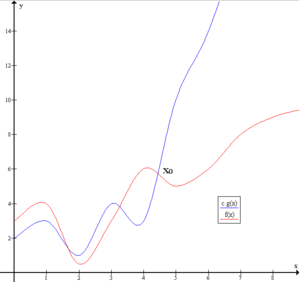
\includegraphics{300px-Big-O-notation.png}
\caption{big Oh notation example}
\end{figure}

\textbf{Example} - \(n^2+13n+43\in \mathcal{O}(n^2)\) -
\(\frac{1}{1000}n^4+10000000n^3+10^{10^{10}}\in \mathcal{O}(n^4)\)

\hypertarget{summation-and-production}{%
\subsubsection{Summation and
Production}\label{summation-and-production}}

\begin{itemize}
\tightlist
\item
  \(\mathcal{O}( f( n)) +\mathcal{O}( g( n)) =\mathcal{O}( f( n) +g( n))\)
\item
  \(\mathcal{O}( f( n)) \times \mathcal{O}( g( n)) =\mathcal{O}( f( n) \times g( n))\)
\item
  \(\mathcal{O}( cf( n)) =\mathcal{O}( f( n))\)
\end{itemize}

\begin{longtable}[]{@{}ccc@{}}
\toprule
\begin{minipage}[b]{0.30\columnwidth}\centering
Notation\strut
\end{minipage} & \begin{minipage}[b]{0.30\columnwidth}\centering
Name\strut
\end{minipage} & \begin{minipage}[b]{0.30\columnwidth}\centering
Example\strut
\end{minipage}\tabularnewline
\midrule
\endhead
\begin{minipage}[t]{0.30\columnwidth}\centering
\[\mathcal{O}(1)\]\strut
\end{minipage} & \begin{minipage}[t]{0.30\columnwidth}\centering
constant\strut
\end{minipage} & \begin{minipage}[t]{0.30\columnwidth}\centering
Determining if a binary number is even or odd\strut
\end{minipage}\tabularnewline
\begin{minipage}[t]{0.30\columnwidth}\centering
\[\mathcal{O}(\log(n))\]\strut
\end{minipage} & \begin{minipage}[t]{0.30\columnwidth}\centering
logarithmic\strut
\end{minipage} & \begin{minipage}[t]{0.30\columnwidth}\centering
Finding an item in a sorted array with a binary search or a balanced
search tree as well as all operations in a Binomial heap\strut
\end{minipage}\tabularnewline
\begin{minipage}[t]{0.30\columnwidth}\centering
\[\mathcal{O}( n)\]\strut
\end{minipage} & \begin{minipage}[t]{0.30\columnwidth}\centering
linear\strut
\end{minipage} & \begin{minipage}[t]{0.30\columnwidth}\centering
Finding an item in an unsorted list\strut
\end{minipage}\tabularnewline
\begin{minipage}[t]{0.30\columnwidth}\centering
\[\mathcal{O}( n\log n) =\mathcal{O}(\log n!)\]\strut
\end{minipage} & \begin{minipage}[t]{0.30\columnwidth}\centering
linearithmic, loglinear, quasilinear\strut
\end{minipage} & \begin{minipage}[t]{0.30\columnwidth}\centering
quick sort\strut
\end{minipage}\tabularnewline
\begin{minipage}[t]{0.30\columnwidth}\centering
\[\mathcal{O}\left(n^{c}\right), _{c >1}\]\strut
\end{minipage} & \begin{minipage}[t]{0.30\columnwidth}\centering
fractional power\strut
\end{minipage} & \begin{minipage}[t]{0.30\columnwidth}\centering
bubble sort(\(c=2\))\strut
\end{minipage}\tabularnewline
\begin{minipage}[t]{0.30\columnwidth}\centering
\[\mathcal{O}\left( c^{n}\right), _{c >1}\]\strut
\end{minipage} & \begin{minipage}[t]{0.30\columnwidth}\centering
exponential\strut
\end{minipage} & \begin{minipage}[t]{0.30\columnwidth}\centering
Finding the (exact) solution to the travelling salesman problem using
dynamic programming; determining if two logical statements are
equivalent using brute-force search\strut
\end{minipage}\tabularnewline
\begin{minipage}[t]{0.30\columnwidth}\centering
\[\mathcal{O}( n!)\]\strut
\end{minipage} & \begin{minipage}[t]{0.30\columnwidth}\centering
factorial\strut
\end{minipage} & \begin{minipage}[t]{0.30\columnwidth}\centering
Solving the travelling salesman problem via brute-force search;
generating all unrestricted permutations of a list\strut
\end{minipage}\tabularnewline
\bottomrule
\end{longtable}

check python operations complexity
\href{https://wiki.python.org/moin/TimeComplexity}{here}

    \hypertarget{recursive-functions}{%
\section{Recursive Functions}\label{recursive-functions}}

    \begin{tcolorbox}[breakable, size=fbox, boxrule=1pt, pad at break*=1mm,colback=cellbackground, colframe=cellborder]
\prompt{In}{incolor}{6}{\boxspacing}
\begin{Verbatim}[commandchars=\\\{\}]
\PY{k}{def} \PY{n+nf}{fact}\PY{p}{(}\PY{n}{n}\PY{p}{)}\PY{p}{:}
    \PY{k}{if} \PY{n}{n}\PY{o}{==}\PY{l+m+mi}{2}\PY{p}{:}
        \PY{k}{return} \PY{l+m+mi}{2}
    \PY{k}{return} \PY{n}{n}\PY{o}{*}\PY{n}{fact}\PY{p}{(}\PY{n}{n}\PY{o}{\PYZhy{}}\PY{l+m+mi}{1}\PY{p}{)}
\PY{n+nb}{print}\PY{p}{(}\PY{n}{fact}\PY{p}{(}\PY{l+m+mi}{50}\PY{p}{)}\PY{p}{)}
\end{Verbatim}
\end{tcolorbox}

    \begin{Verbatim}[commandchars=\\\{\}]
30414093201713378043612608166064768844377641568960512000000000000
    \end{Verbatim}

    This function works in \(\mathcal{O}(n)\)

    \begin{tcolorbox}[breakable, size=fbox, boxrule=1pt, pad at break*=1mm,colback=cellbackground, colframe=cellborder]
\prompt{In}{incolor}{7}{\boxspacing}
\begin{Verbatim}[commandchars=\\\{\}]
\PY{k}{def} \PY{n+nf}{fib0}\PY{p}{(}\PY{n}{n}\PY{p}{)}\PY{p}{:}
    \PY{k}{if} \PY{n}{n} \PY{o+ow}{in} \PY{p}{[}\PY{l+m+mi}{2}\PY{p}{,}\PY{l+m+mi}{1}\PY{p}{]}\PY{p}{:}
        \PY{k}{return} \PY{l+m+mi}{1}
    \PY{k}{return} \PY{n}{fib0}\PY{p}{(}\PY{n}{n}\PY{o}{\PYZhy{}}\PY{l+m+mi}{1}\PY{p}{)}\PY{o}{+}\PY{n}{fib0}\PY{p}{(}\PY{n}{n}\PY{o}{\PYZhy{}}\PY{l+m+mi}{2}\PY{p}{)}

\PY{k}{def} \PY{n+nf}{fib1}\PY{p}{(}\PY{n}{n}\PY{p}{)}\PY{p}{:}
    \PY{n}{a}\PY{p}{,}\PY{n}{b}\PY{o}{=}\PY{l+m+mi}{1}\PY{p}{,}\PY{l+m+mi}{1}
    \PY{k}{for} \PY{n}{i} \PY{o+ow}{in} \PY{n+nb}{range}\PY{p}{(}\PY{n}{n}\PY{o}{\PYZhy{}}\PY{l+m+mi}{1}\PY{p}{)}\PY{p}{:}
        \PY{n}{a}\PY{p}{,}\PY{n}{b} \PY{o}{=} \PY{n}{b}\PY{p}{,}\PY{n}{a}\PY{o}{+}\PY{n}{b}
    \PY{k}{return} \PY{n}{b}
\PY{n+nb}{print}\PY{p}{(}\PY{n}{fib0}\PY{p}{(}\PY{l+m+mi}{10}\PY{p}{)}\PY{p}{)}
\PY{n+nb}{print}\PY{p}{(}\PY{n}{fib1}\PY{p}{(}\PY{l+m+mi}{10}\PY{p}{)}\PY{p}{)}
\end{Verbatim}
\end{tcolorbox}

    \begin{Verbatim}[commandchars=\\\{\}]
55
89
    \end{Verbatim}

    \textbf{Question:} find the complexity of both functions

    \hypertarget{arrays}{%
\section{Arrays}\label{arrays}}

\textbf{a contiguous area of memory} that is one chunk of memory that
can either be on the stack or it can be in the heap, doesn't really
matter where it is. It is broken down into \textbf{equal-sized
elements}, and each of those elements are \textbf{indexed by contiguous
integers}.

    \hypertarget{why-arrays-are-important}{%
\subsection{Why Arrays are Important?}\label{why-arrays-are-important}}

the address of our particular array element is: \[
array\_addr+ elem\_size \times (i-first\_index)
\]

\begin{longtable}[]{@{}cll@{}}
\toprule
memory address & value & index\tabularnewline
\midrule
\endhead
100 & 4 & 0\tabularnewline
104 & 5 & 1\tabularnewline
108 & 67 & 2\tabularnewline
112 & 8 & 3\tabularnewline
116 & 9 & 4\tabularnewline
120 & 2 & 5\tabularnewline
\bottomrule
\end{longtable}

    \begin{tcolorbox}[breakable, size=fbox, boxrule=1pt, pad at break*=1mm,colback=cellbackground, colframe=cellborder]
\prompt{In}{incolor}{8}{\boxspacing}
\begin{Verbatim}[commandchars=\\\{\}]
\PY{k+kn}{from} \PY{n+nn}{array} \PY{k+kn}{import} \PY{n}{array}
\PY{n}{arr} \PY{o}{=} \PY{n}{array}\PY{p}{(}\PY{l+s+s1}{\PYZsq{}}\PY{l+s+s1}{i}\PY{l+s+s1}{\PYZsq{}}\PY{p}{,}\PY{p}{[}\PY{l+m+mi}{4}\PY{p}{,}\PY{l+m+mi}{5}\PY{p}{,}\PY{l+m+mi}{67}\PY{p}{,}\PY{l+m+mi}{8}\PY{p}{,}\PY{l+m+mi}{9}\PY{p}{,}\PY{l+m+mi}{2}\PY{p}{]}\PY{p}{)}
\PY{n}{buffer\PYZus{}info} \PY{o}{=} \PY{n}{arr}\PY{o}{.}\PY{n}{buffer\PYZus{}info}\PY{p}{(}\PY{p}{)}
\PY{n+nb}{print}\PY{p}{(}\PY{l+s+sa}{f}\PY{l+s+s2}{\PYZdq{}}\PY{l+s+si}{\PYZob{}}\PY{n}{buffer\PYZus{}info}\PY{l+s+si}{=\PYZcb{}}\PY{l+s+s2}{\PYZdq{}}\PY{p}{)}
\PY{n+nb}{print}\PY{p}{(}\PY{n+nb}{hex}\PY{p}{(}\PY{n}{buffer\PYZus{}info}\PY{p}{[}\PY{l+m+mi}{0}\PY{p}{]}\PY{p}{)}\PY{p}{)}
\end{Verbatim}
\end{tcolorbox}

    \begin{Verbatim}[commandchars=\\\{\}]
buffer\_info=(140304787604656, 6)
0x7f9b410684b0
    \end{Verbatim}

    \hypertarget{two-dimensional-arrays}{%
\subsection{Two Dimensional Arrays}\label{two-dimensional-arrays}}

\[
\displaystyle \begin{bmatrix}
a_{00} & a_{01} & a_{02} & a_{03}\\
a_{10} & a_{11} & a_{12} & a_{13}\\
a_{20} & a_{21} & a_{22} & a_{23}\\
a_{30} & a_{31} & a_{32} & a_{33}
\end{bmatrix}
\]

\hypertarget{row-major}{%
\subsubsection{Row-major}\label{row-major}}

\[
\begin{bmatrix}
a_{00} & a_{01} & a_{02} & a_{03} & a_{10} & a_{11} & a_{12} & a_{13}& a_{20} & a_{21} & a_{22} & a_{23} & a_{30} & a_{31} & a_{32} & a_{33}
\end{bmatrix}
\]

Now to access \(a_{ij}\) for \(M\times N\) matrix: \[
array\_adr + elem\_size (M(i-I)+(j-J))
\]

\hypertarget{column-major}{%
\subsubsection{Column-major}\label{column-major}}

\[
\begin{bmatrix}
a_{00} & a_{10} & a_{20} & a_{30} & a_{01} & a_{11} & a_{21} & a_{31}& a_{02} & a_{12} & a_{22} & a_{32}& a_{03} & a_{13} & a_{23} & a_{33}
\end{bmatrix}
\]

Now to access \(a_{ij}\) for \(M\times N\) matrix: \[
array\_adr + elem\_size ((i-I)+N(j-J))
\]

    \hypertarget{homeworks}\DecValTok{10} \OperatorTok{==} \DecValTok{0}\NormalTok{:}
\NormalTok{        nfact}\OperatorTok{/=}\DecValTok{10}
\NormalTok{        counter}\OperatorTok{+=}\DecValTok{1}
    \ControlFlowTok{return}\NormalTok{ counter}
\end{Highlighting}
\end{Shaded}

And:

\begin{Shaded}
\begin{Highlighting}[]
\KeywordTok{def}\NormalTok{ findLastZeros1(n):}
\NormalTok{    counter }\OperatorTok{=} \DecValTok{0}
\NormalTok{    t }\OperatorTok{=} \DecValTok{1}
    \ControlFlowTok{for}\NormalTok{ i }\KeywordTok{in} \BuiltInTok{str}\NormalTok{(fact(n))[::}\OperatorTok{-}\DecValTok{1}\NormalTok{]:}
\NormalTok{        t }\OperatorTok{=} \BuiltInTok{int}\NormalTok{(i)}\OperatorTok{%}\DecValTok{11}
\NormalTok{        counter}\OperatorTok{+=}\NormalTok{t}
    \ControlFlowTok{return}\NormalTok{ counter}
\end{Highlighting}
\end{Shaded}

Or this is as same as:

\begin{Shaded}
\begin{Highlighting}[]
\KeywordTok{def}\NormalTok{ findLastZeros2(n):}
\NormalTok{    t}\OperatorTok{=}\DecValTok{1}
    \ControlFlowTok{return} \BuiltInTok{sum}\NormalTok{((t:}\OperatorTok{=}\BuiltInTok{int}\NormalTok{(i}\OperatorTok{==}\StringTok{'0'} \KeywordTok{and}\NormalTok{ t)) }\ControlFlowTok{for}\NormalTok{ i }\KeywordTok{in} \BuiltInTok{str}\NormalTok{(fact(n))[::}\OperatorTok{-}\DecValTok{1}\NormalTok{])}
\end{Highlighting}
\end{Shaded}

your task is to: 1. find the time complexity of these functions, and
find out wich one is faster 2. find a faster way to compute same value

    \begin{tcolorbox}[breakable, size=fbox, boxrule=1pt, pad at break*=1mm,colback=cellbackground, colframe=cellborder]
\prompt{In}{incolor}{9}{\boxspacing}
\begin{Verbatim}[commandchars=\\\{\}]
\PY{k}{def} \PY{n+nf}{findLastZeros0}\PY{p}{(}\PY{n}{n}\PY{p}{)}\PY{p}{:}
    \PY{n}{nfact}\PY{o}{=}\PY{n}{fact}\PY{p}{(}\PY{n}{n}\PY{p}{)}
    \PY{n}{counter} \PY{o}{=} \PY{l+m+mi}{0}
    \PY{k}{while} \PY{n}{nfact}\PY{o}{\PYZpc{}}\PY{k}{10} == 0:
        \PY{n}{nfact}\PY{o}{/}\PY{o}{/}\PY{o}{=}\PY{l+m+mi}{10}
        \PY{n}{counter}\PY{o}{+}\PY{o}{=}\PY{l+m+mi}{1}
    \PY{k}{return} \PY{n}{counter}
\PY{k}{def} \PY{n+nf}{findLastZeros1}\PY{p}{(}\PY{n}{n}\PY{p}{)}\PY{p}{:}
    \PY{n}{counter} \PY{o}{=} \PY{l+m+mi}{0}
    \PY{n}{t} \PY{o}{=} \PY{l+m+mi}{1}
    \PY{k}{for} \PY{n}{i} \PY{o+ow}{in} \PY{n+nb}{str}\PY{p}{(}\PY{n}{fact}\PY{p}{(}\PY{n}{n}\PY{p}{)}\PY{p}{)}\PY{p}{[}\PY{p}{:}\PY{p}{:}\PY{o}{\PYZhy{}}\PY{l+m+mi}{1}\PY{p}{]}\PY{p}{:}
        \PY{n}{t} \PY{o}{=} \PY{n+nb}{int}\PY{p}{(}\PY{n}{i}\PY{o}{==}\PY{l+s+s1}{\PYZsq{}}\PY{l+s+s1}{0}\PY{l+s+s1}{\PYZsq{}} \PY{o+ow}{and} \PY{n}{t}\PY{p}{)}
        \PY{n}{counter}\PY{o}{+}\PY{o}{=}\PY{n}{t}
    \PY{k}{return} \PY{n}{counter}

\PY{k}{def} \PY{n+nf}{findLastZeros2}\PY{p}{(}\PY{n}{n}\PY{p}{)}\PY{p}{:}
    \PY{n}{t}\PY{o}{=}\PY{l+m+mi}{1}
    \PY{k}{return} \PY{n+nb}{sum}\PY{p}{(}\PY{p}{(}\PY{n}{t}\PY{o}{:=}\PY{n+nb}{int}\PY{p}{(}\PY{n}{i}\PY{o}{==}\PY{l+s+s1}{\PYZsq{}}\PY{l+s+s1}{0}\PY{l+s+s1}{\PYZsq{}} \PY{o+ow}{and} \PY{n}{t}\PY{p}{)}\PY{p}{)} \PY{k}{for} \PY{n}{i} \PY{o+ow}{in} \PY{n+nb}{str}\PY{p}{(}\PY{n}{fact}\PY{p}{(}\PY{n}{n}\PY{p}{)}\PY{p}{)}\PY{p}{[}\PY{p}{:}\PY{p}{:}\PY{o}{\PYZhy{}}\PY{l+m+mi}{1}\PY{p}{]}\PY{p}{)}

\PY{n+nb}{print}\PY{p}{(}\PY{l+s+sa}{f}\PY{l+s+s2}{\PYZdq{}}\PY{l+s+si}{\PYZob{}}\PY{n}{fact}\PY{p}{(}\PY{l+m+mi}{30}\PY{p}{)}\PY{l+s+si}{=\PYZcb{}}\PY{l+s+s2}{\PYZdq{}}\PY{p}{)}
\PY{n+nb}{print}\PY{p}{(}\PY{l+s+sa}{f}\PY{l+s+s2}{\PYZdq{}}\PY{l+s+si}{\PYZob{}}\PY{n}{findLastZeros0}\PY{p}{(}\PY{l+m+mi}{30}\PY{p}{)}\PY{l+s+si}{=\PYZcb{}}\PY{l+s+s2}{\PYZdq{}}\PY{p}{)}
\PY{n+nb}{print}\PY{p}{(}\PY{l+s+sa}{f}\PY{l+s+s2}{\PYZdq{}}\PY{l+s+si}{\PYZob{}}\PY{n}{findLastZeros1}\PY{p}{(}\PY{l+m+mi}{30}\PY{p}{)}\PY{l+s+si}{=\PYZcb{}}\PY{l+s+s2}{\PYZdq{}}\PY{p}{)}
\PY{n+nb}{print}\PY{p}{(}\PY{l+s+sa}{f}\PY{l+s+s2}{\PYZdq{}}\PY{l+s+si}{\PYZob{}}\PY{n}{findLastZeros2}\PY{p}{(}\PY{l+m+mi}{30}\PY{p}{)}\PY{l+s+si}{=\PYZcb{}}\PY{l+s+s2}{\PYZdq{}}\PY{p}{)}
\end{Verbatim}
\end{tcolorbox}

    \begin{Verbatim}[commandchars=\\\{\}]
fact(30)=265252859812191058636308480000000
findLastZeros0(30)=7
findLastZeros1(30)=7
findLastZeros2(30)=7
    \end{Verbatim}

    \textbf{Question2:} implement two functions to convert two-dimensional
array to one-dimensional and vise versa here is a template code for you.

    \begin{tcolorbox}[breakable, size=fbox, boxrule=1pt, pad at break*=1mm,colback=cellbackground, colframe=cellborder]
\prompt{In}{incolor}{10}{\boxspacing}
\begin{Verbatim}[commandchars=\\\{\}]
\PY{k}{def} \PY{n+nf}{\PYZus{}2Dto1D}\PY{p}{(}\PY{n}{arr}\PY{p}{,}\PY{n}{method}\PY{o}{=}\PY{l+s+s1}{\PYZsq{}}\PY{l+s+s1}{Row\PYZhy{}major}\PY{l+s+s1}{\PYZsq{}}\PY{p}{)}\PY{p}{:}
    \PY{k}{if} \PY{n}{method} \PY{o+ow}{not} \PY{o+ow}{in} \PY{p}{[}\PY{l+s+s1}{\PYZsq{}}\PY{l+s+s1}{Row\PYZhy{}major}\PY{l+s+s1}{\PYZsq{}}\PY{p}{,}\PY{l+s+s1}{\PYZsq{}}\PY{l+s+s1}{Col\PYZhy{}major}\PY{l+s+s1}{\PYZsq{}}\PY{p}{]}\PY{p}{:}
        \PY{k}{raise} \PY{n+ne}{ValueError}\PY{p}{(}\PY{l+s+sa}{f}\PY{l+s+s2}{\PYZdq{}}\PY{l+s+s2}{mathod must be either }\PY{l+s+s2}{\PYZsq{}}\PY{l+s+s2}{Row\PYZhy{}major}\PY{l+s+s2}{\PYZsq{}}\PY{l+s+s2}{ or }\PY{l+s+s2}{\PYZsq{}}\PY{l+s+s2}{Col\PYZhy{}major}\PY{l+s+s2}{\PYZsq{}}\PY{l+s+s2}{ not }\PY{l+s+si}{\PYZob{}}\PY{n}{method}\PY{l+s+si}{\PYZcb{}}\PY{l+s+s2}{\PYZdq{}}\PY{p}{)}
    \PY{c+c1}{\PYZsh{} write your code}

\PY{k}{def} \PY{n+nf}{\PYZus{}1Dto2D}\PY{p}{(}\PY{n}{arr}\PY{p}{,}\PY{n}{n}\PY{p}{,}\PY{n}{m}\PY{p}{,}\PY{n}{method}\PY{o}{=}\PY{l+s+s1}{\PYZsq{}}\PY{l+s+s1}{Row\PYZhy{}major}\PY{l+s+s1}{\PYZsq{}}\PY{p}{)}\PY{p}{:}
    \PY{k}{assert} \PY{n}{method} \PY{o+ow}{in} \PY{p}{[}\PY{l+s+s1}{\PYZsq{}}\PY{l+s+s1}{Row\PYZhy{}major}\PY{l+s+s1}{\PYZsq{}}\PY{p}{,}\PY{l+s+s1}{\PYZsq{}}\PY{l+s+s1}{Col\PYZhy{}major}\PY{l+s+s1}{\PYZsq{}}\PY{p}{]}\PY{p}{,} \PY{l+s+sa}{f}\PY{l+s+s2}{\PYZdq{}}\PY{l+s+s2}{method must be either }\PY{l+s+s2}{\PYZsq{}}\PY{l+s+s2}{Row\PYZhy{}major}\PY{l+s+s2}{\PYZsq{}}\PY{l+s+s2}{ or }\PY{l+s+s2}{\PYZsq{}}\PY{l+s+s2}{Col\PYZhy{}major}\PY{l+s+s2}{\PYZsq{}}\PY{l+s+s2}{ not }\PY{l+s+si}{\PYZob{}}\PY{n}{method}\PY{l+s+si}{\PYZcb{}}\PY{l+s+s2}{\PYZdq{}}
    \PY{k}{assert} \PY{n}{n}\PY{o}{*}\PY{n}{m}\PY{o}{==}\PY{n+nb}{len}\PY{p}{(}\PY{n}{arr}\PY{p}{)}\PY{p}{,} \PY{l+s+sa}{f}\PY{l+s+s2}{\PYZdq{}}\PY{l+s+si}{\PYZob{}}\PY{n}{n}\PY{o}{*}\PY{n}{m}\PY{l+s+si}{=\PYZcb{}}\PY{l+s+s2}{ which must be }\PY{l+s+si}{\PYZob{}}\PY{n+nb}{len}\PY{p}{(}\PY{n}{arr}\PY{p}{)}\PY{l+s+si}{\PYZcb{}}\PY{l+s+s2}{\PYZdq{}}
    \PY{c+c1}{\PYZsh{} write your code here}
\end{Verbatim}
\end{tcolorbox}


    % Add a bibliography block to the postdoc



\end{document}
